% samples/figures-test.tex – renders every finished figure in the book's typography (P5 check).
\documentclass{smartcross}
% samples/meta.tex – shared metadata for the design samples (same as main.tex)
\Title{חוצים באדום}
\Subtitle{מעבר חצייה חכם: אדום אדפטיבי, ספירה לאחור בזמן הפינוי ושליטה חברתית}
\EnglishTitle{Crossing at a Red Light – Smart Pedestrian Crossing: A Preparatory Report}
\Institution{אוניברסיטת בר-אילן}
\Course{בינה מלאכותית יוצרת: מודלי שפה, סוכנים ומערכות מרובות סוכנים}
\Lecturer{ד״ר יורם סגל}
\Authors{קבוצת \en{shirloma}}
\DocDate{נובמבר \num{2026}}
\GroupCode{shirloma}
\FooterTitle{חוצים באדום}
\DocNumber{SCX-PR-001}
\DocRevision{0.1}
\addbibresource{references/refs.bib}

\begin{document}
\MainMatter
\ChapterMission{בדיקת איורים: כל איור מוצג בגודל ובגופן של הספר}
\chapter{בדיקת איורים}
\begin{scenebox}
דף בדיקה פנימי לאיורים בלבד.
\end{scenebox}
האיורים \ref{fig:t1}, \ref{fig:g1}, \ref{fig:g2} ו-\ref{fig:g3} מוצגים כאן לבדיקה בלבד.
\begin{figure}[ht]\centering
  \begin{ltrblock}\centering% T1 – the smart crossing in plan view: waiting zone, curb sensing zone, countdown heads, controller, awareness display.
% LTR coordinates; every Hebrew node uses the 'rtl' style (DS-01). Colours/pictograms from smartcross.cls only.
\begin{tikzpicture}[x=1mm,y=1mm,
  lab/.style={rtl,font=\sffamily\fontsize{7.5}{9.5}\selectfont,text=Asphalt,align=flush right,inner sep=1pt},
  lead/.style={AsphaltLight,line width=0.4pt},
  link/.style={SignalAmber!85!black,line width=0.7pt,dash pattern=on 2pt off 1.4pt}]
  % sidewalks, curbs, road
  \fill[Concrete] (0,50) rectangle (134,64);  \fill[Concrete] (0,0) rectangle (134,12);
  \fill[Curb] (0,49) rectangle (134,50);       \fill[Curb] (0,12) rectangle (134,13);
  \fill[Road] (0,13) rectangle (134,49);
  \foreach \x in {2,12,...,40}{\fill[StripeWhite,opacity=.7] (\x,30.6) rectangle ++(6,.8);}
  \foreach \x in {94,104,...,130}{\fill[StripeWhite,opacity=.7] (\x,30.6) rectangle ++(6,.8);}
  \foreach \i in {0,...,6}{\fill[StripeWhite] (52,{15.5+\i*4.9}) rectangle (82,{17.9+\i*4.9});}
  % waiting zone + sensing fan (far curb)
  \fill[SignalAmber,opacity=.16] (88,52) -- ++(180:34) arc[start angle=180,end angle=160,radius=34] -- cycle;
  \draw[SignalAmber!85!black,line width=.5pt,dash pattern=on 2pt off 1.4pt] (88,52) -- ++(180:34) arc[start angle=180,end angle=160,radius=34] -- cycle;
  \draw[Asphalt,line width=.5pt,dash pattern=on 1pt off 1pt] (54,51) rectangle (80,62);
  \foreach \x/\y in {58/57,63/59,68/56,73/58.5}{\fill[Asphalt] (\x,\y) circle (1.1); \fill[AsphaltLight] (\x,\y-1.9) ellipse (2 and .9);}
  \fill[HousingBlack] (88,52) circle (1.4); \fill[SignalAmber] (88,52) circle (.6);
  % countdown signal heads (both curbs)
  \foreach \x/\y in {86/57,48/5}{
    \fill[HousingBlack,rounded corners=.8] (\x-3,\y-2.5) rectangle (\x+3,\y+5.5);
    \node[inner sep=0] at (\x,\y+3) {\fontsize{6}{6}\selectfont\picto[SignalRed]{pedestrian}};
    \node[inner sep=0,text=SignalAmber,font=\sffamily\bfseries\fontsize{5.5}{5.5}\selectfont] at (\x,\y-0.6) {12};}
  % awareness display (near curb) and controller cabinet
  \fill[Asphalt,rounded corners=.8] (88,3) rectangle (104,9); \node[inner sep=0,text=StripeWhite,font=\sffamily\bfseries\fontsize{5}{5}\selectfont] at (96,6) {\num{4}~\picto[StripeWhite]{pedestrian}};
  \fill[AsphaltDeep,rounded corners=.8] (112,2) rectangle (126,10); \node[inner sep=0] at (119,6) {\fontsize{7}{7}\selectfont\picto[SignalAmber]{signal}};
  % data links to the controller
  \draw[link] (119,10) -- (119,52) -- (89.6,52);
  \draw[link] (119,52) |- (89,57);
  \draw[link] (112,6) -- (104,6);
  \draw[link] (112,4) -- (51,4) -- (51,5);
  % callouts (Hebrew, RTL)
  \draw[lead] (67,62) -- (67,68.5); \node[lab,anchor=south] at (67,68.8) {אזור המתנה};
  \draw[lead] (57,55) -- (32,55) -- (32,68.5); \node[lab,anchor=south] at (32,68.8) {אזור חישה (מונה ממתינים)};
  \draw[lead] (86,63) -- (86,64.5) -- (106,64.5) -- (106,68.5); \node[lab,anchor=south] at (106,68.8) {ראש רמזור עם ספירה לאחור};
  \draw[lead] (67,13.5) -- (67,-4); \node[lab,anchor=north] at (67,-4) {מעבר חציה};
  \draw[lead] (96,3) -- (96,-4); \node[lab,anchor=north] at (96,-4) {שלט מודעות};
  \draw[lead] (119,2) -- (119,-4); \node[lab,anchor=north] at (121,-4) {בקר הרמזור};
  \draw[link] (4,-7.5) -- ++(7,0); \node[lab,anchor=west] at (12,-7.5) {קישור נתונים};
\end{tikzpicture}
\end{ltrblock}
  \caption{מעבר החצייה החכם במבט על: אזור ההמתנה, אזור החישה, ראשי הרמזור עם ספירה לאחור, שלט המודעות והבקר}\label{fig:t1}
\end{figure}
\begin{figure}[ht]\centering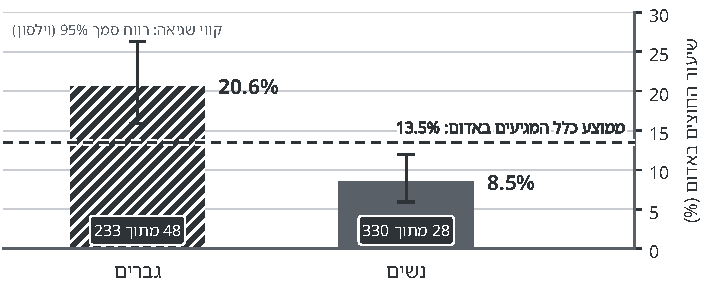
\includegraphics[width=\linewidth]{figures/g1-crossing-by-gender.pdf}
  \caption{שיעור החצייה באדום בקרב המגיעים במופע האדום, לפי מגדר (עובד מתוך \cite{rosenbloom2009})}\label{fig:g1}\end{figure}
\begin{figure}[ht]\centering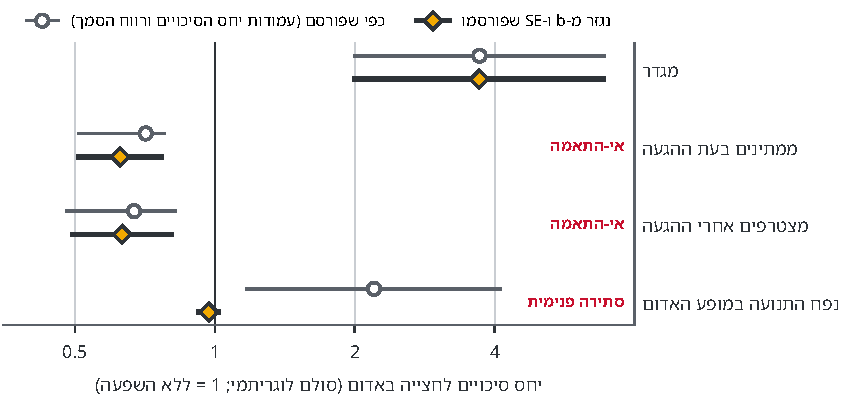
\includegraphics[width=\linewidth]{figures/g2-odds-ratios.pdf}
  \caption{יחסי הסיכויים בטבלה 2 של המקור: כפי שפורסמו ולאחר חישוב מחדש (עובד מתוך \cite{rosenbloom2009})}\label{fig:g2}\end{figure}
\begin{figure}[ht]\centering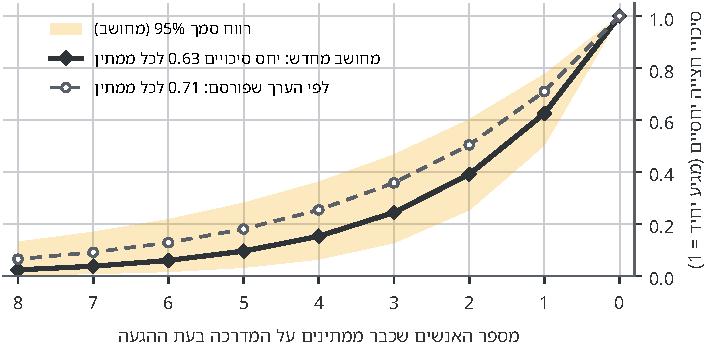
\includegraphics[width=\linewidth]{figures/g3-relative-odds.pdf}
  \caption{סיכויי החצייה היחסיים לפי מספר הממתינים (חושב מתוך \cite{rosenbloom2009})}\label{fig:g3}\end{figure}
\end{document}
